\section{Results}
\subsection{Setup}
We used \textit{Mininet}~\cite{conf/hotnets/LantzHM10, Mininet} to emulate a software-defined network environment and \textit{Open vSwitch}~\cite{Pfaff2009, OVS} as the OpenFlow enabled switch. \textit{Ryu} SDN framework~\cite{Ryu} was used to build the monitoring application in Python. The setup of the experiments used to evaluate the performance of the algorithms on local node problems was a single switch connected to two hosts via different ports, and the routing entries were set to simply forward traffic from one port to the other.

\textit{Tcpreplay}\footnote{Pcap editing and replaying utilities. available at: http://tcpreplay.appneta.com} was used to replay CAIDA traffic trace~\cite{CAIDA14, CAIDA16} into the network. Considering the prefixing nature of the algorithm, in order to keep the original characteristics of the real traffic and the privacy of the users, one should be careful to use real traffic traces that went through ``prefix-preserving anonymization'' such as the CAIDA traces.

The traces replayed into the network were slowed down by a factor of $11$ in order to allow the software to cope with the high rate of the recorded traffic and avoid dropping events. Therefore, all timing aspects of the experiments were slowed down by the same factor, and the results are reported in the real timing values rather than the actual ones.

For the evaluation we used two CAIDA traces, from 2014 and 2016\footnote{Data from 2015 was used in the comparison to RAP.}, considering 1-minute interval. The CAIDA'14 trace has the property that the top-$15$ flows are the same $15$ flow throughout every 12-second interval in this minute.
On the other hand, the CAIDA'16 trace has a very significant heavy flow over the whole minute, while the next heaviest flows vary depending on which subinterval is considered. In this sense, the CAIDA'16 trace is an adversarial input due to lack of consistent heavy flows throughout the monitoring intervals.

\subsection{Evaluation of local top-$k$ algorithms}
First, we evaluated the performance of the algorithm \ref{algo:BasicSplitting} on both traces. For that, we conducted a series of experiments to solve $ApproxTop(S,k,\varepsilon)$, with different values of $k$ and $m$ using traffic from both datasets and a constant $\varepsilon=0.05$.

To quantify the performance of the algorithms we define the approximate top-$k$ set ($ATk$), to be the set of flows with frequency higher than $(1-\varepsilon)n_k$, where $n_k$ is the frequency of the $k^{th}$ heaviest flow.
Then the \textit{Detection Rate (DR)} is the percentage of approximate top-$k$ flows the algorithm managed to detect, i.e., $DR=\frac{|f\in output\cap ATk|}{k}$. We note that since all algorithms output exactly $k$ flows, the detection rate is at most $1$.

Figure~\ref{fig:km2014-DR1} depicts the effect of $k$ and $m$ on the detection rate of the algorithm \ref{algo:BasicSplitting} using the CAIDA'14 traces. It is evident that for small values of $k$ the algorithm performs well, achieving a detection rate of at least $0.9$. As expected, for a given number of counters, increasing $k$ decreases the detection rate.
Furthermore, one can see that as the value of $m$ increases the detection rate for a given $k$ also increases, which is expected since the algorithm is using more counters to detect the same heaviest top-$k$ flows.

As expected, when considering experiments with the adversarial traces of CAIDA'16, the performance degrades as seen in Figure~\ref{fig:kmBoth-DR1}. For example, the perfect detection rate for $k=8$ decreases to just above 86\%. Furthermore, the algorithm now needs $128$ counters instead of $32$ to achieve a detection rate about 85\% for $k=12$.

% \begin{figure}
% \subfloat[CAIDA'14 traces \label{fig:km2014-DR1}]{
% \resizebox {0.5\columnwidth} {!} {
% \begin{tikzpicture}
%     \begin{axis}[
%     xlabel={Number of Counters},
%     ylabel={Detection Rate},
%     xtick=data,
%     xticklabels={32, 64, 128, 512},
%     ytick={50,55,60,65,70,75,80,85,90,95,100},
%     legend pos=south east,
%     legend columns=2,
%     ymajorgrids=true,
%     grid style=dashed
%     ]
%     \addplot+[black, mark=o]
%     coordinates {
%         (1,100)(2,100)(3,100)(4,100)
%     };
%     \addlegendentry{$k$=8};
%     \addplot+[black, mark=x]
%     coordinates {
%         (1,90)(2,90)(3,92.5)(4,95)
%     };
%     \addlegendentry{$k$=10};
%     \addplot+[black, mark=|]
%     coordinates {
%         (1,83.3)(2,87.5)(3,85.41)(4,85.41)
%     };
%     \addlegendentry{$k$=12};
%     \addplot+[black, mark=square]
%     coordinates {
%         (1,68.9)(2,75)(3,81.67)(4,83.33)
%     };
%     \addlegendentry{$k$=15};
%     \addplot+[black, mark=triangle]
%     coordinates {
%         (1,61.6)(2,67.5)(3,73.75)(4,77.5)
%     };
%     \addlegendentry{$k$=20};
%     \addplot+[black, mark=diamond]
%     coordinates {
%         (1,58.32)(2,66)(3,75)(4,78)
%     };
%     \addlegendentry{$k$=25};
%     \addplot+[black, mark=pentagon]
%     coordinates {
%         (1,50)(2,67.96)(3,75)(4,75.75)
%     };
%     \addlegendentry{$k$=32};
%     \end{axis}
%     \end{tikzpicture}
% }
% }
% \subfloat[CAIDA'14 + CAIDA'16 traces \label{fig:kmBoth-DR1}]{
% \resizebox {0.5\columnwidth} {!} {
% \begin{tikzpicture}
%     \begin{axis}[
%     xlabel={Number of Counters},
%     ylabel={Detection Rate},
%     xtick=data,
%     xticklabels={32, 64, 128, 512},
%     ytick={40,45,50,55,60,65,70,75,80,85,90},
%     legend pos=south east,
%     legend columns=2,
%     ymajorgrids=true,
%     grid style=dashed
%     ]
%     \addplot+[black, mark=o]
%     coordinates {
%         (1,85)(2,81.25)(3,85.93)(4,84.375)
%     };
%     \addlegendentry{$k$=8};
%     \addplot+[black, mark=x]
%     coordinates {
%         (1,78)(2,78.89)(3,82.5)(4,83.75)
%     };
%     \addlegendentry{$k$=10};
%     \addplot+[black, mark=|]
%     coordinates {
%         (1,73.24)(2,78.125)(3,82.29)(4,83.33)
%     };
%     \addlegendentry{$k$=12};
%     \addplot+[black, mark=square]
%     coordinates {
%         (1,60)(2,68.33)(3,76.67)(4,78.33)
%     };
%     \addlegendentry{$k$=15};
%     \addplot+[black, mark=triangle]
%     coordinates {
%         (1,53)(2,60)(3,70.625)(4,73.75)
%     };
%     \addlegendentry{$k$=20};
%     \addplot+[black, mark=diamond]
%     coordinates {
%         (1,48.36)(2,56)(3,70)(4,73.5)
%     };
%     \addlegendentry{$k$=25};
%     \addplot+[black, mark=pentagon]
%     coordinates {
%         (1,40)(2,52.73)(3,65.23)(4,70.31)
%     };
%     \addlegendentry{$k$=32};
%     \end{axis}
%     \end{tikzpicture}
% }
% }
% \caption{Effects of $k$ and $m$ on the detection rate of Algorithm \ref{algo:BasicSplitting}}
% \end{figure}

\begin{figure}
    \centering
    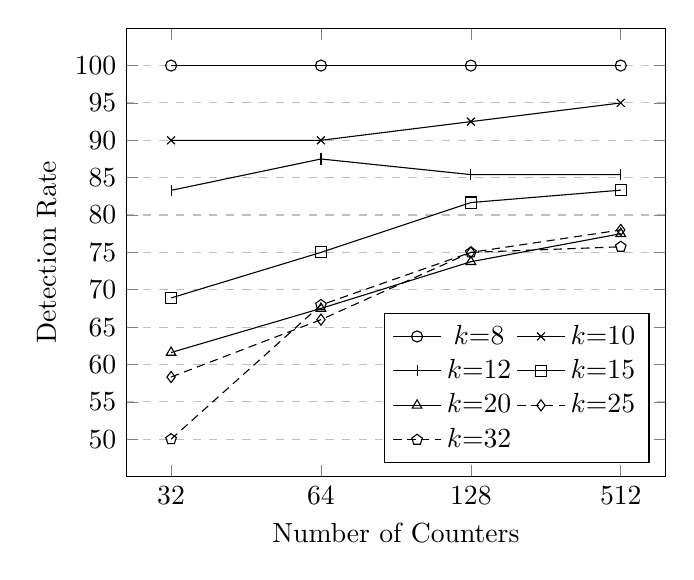
\begin{tikzpicture}
    \begin{axis}[
    xlabel={Number of Counters},
    ylabel={Detection Rate},
    xtick=data,
    xticklabels={32, 64, 128, 512},
    ytick={50,55,60,65,70,75,80,85,90,95,100},
    legend pos=south east,
    legend columns=2,
    ymajorgrids=true,
    grid style=dashed
    ]
    \addplot+[black, mark=o]
    coordinates {
        (1,100)(2,100)(3,100)(4,100)
    };
    \addlegendentry{$k$=8};
    \addplot+[black, mark=x]
    coordinates {
        (1,90)(2,90)(3,92.5)(4,95)
    };
    \addlegendentry{$k$=10};
    \addplot+[black, mark=|]
    coordinates {
        (1,83.3)(2,87.5)(3,85.41)(4,85.41)
    };
    \addlegendentry{$k$=12};
    \addplot+[black, mark=square]
    coordinates {
        (1,68.9)(2,75)(3,81.67)(4,83.33)
    };
    \addlegendentry{$k$=15};
    \addplot+[black, mark=triangle]
    coordinates {
        (1,61.6)(2,67.5)(3,73.75)(4,77.5)
    };
    \addlegendentry{$k$=20};
    \addplot+[black, mark=diamond]
    coordinates {
        (1,58.32)(2,66)(3,75)(4,78)
    };
    \addlegendentry{$k$=25};
    \addplot+[black, mark=pentagon]
    coordinates {
        (1,50)(2,67.96)(3,75)(4,75.75)
    };
    \addlegendentry{$k$=32};
    \end{axis}
    \end{tikzpicture}
    \caption{Effects of $k$ and $m$ on the detection rate of Algorithm \ref{algo:BasicSplitting} - CAIDA'14 traces.}
    \label{fig:km2014-DR1}
\end{figure}

\begin{figure}
    \centering
    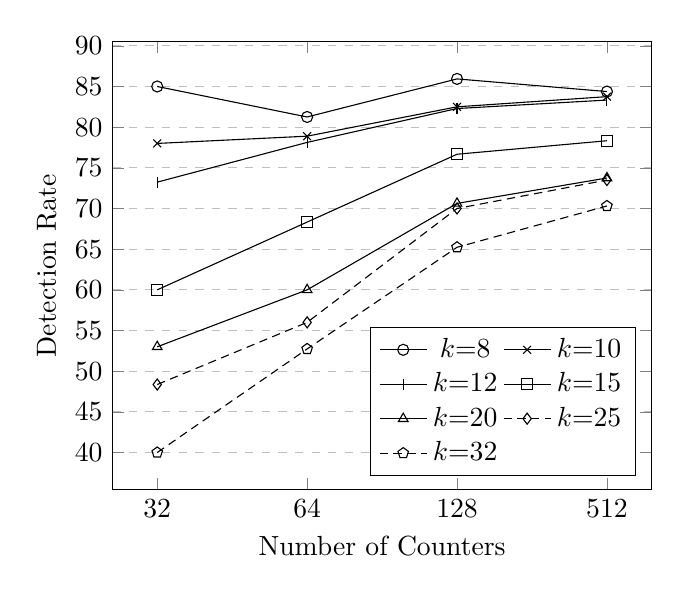
\begin{tikzpicture}
    \begin{axis}[
    xlabel={Number of Counters},
    ylabel={Detection Rate},
    xtick=data,
    xticklabels={32, 64, 128, 512},
    ytick={40,45,50,55,60,65,70,75,80,85,90},
    legend pos=south east,
    legend columns=2,
    ymajorgrids=true,
    grid style=dashed
    ]
    \addplot+[black, mark=o]
    coordinates {
        (1,85)(2,81.25)(3,85.93)(4,84.375)
    };
    \addlegendentry{$k$=8};
    \addplot+[black, mark=x]
    coordinates {
        (1,78)(2,78.89)(3,82.5)(4,83.75)
    };
    \addlegendentry{$k$=10};
    \addplot+[black, mark=|]
    coordinates {
        (1,73.24)(2,78.125)(3,82.29)(4,83.33)
    };
    \addlegendentry{$k$=12};
    \addplot+[black, mark=square]
    coordinates {
        (1,60)(2,68.33)(3,76.67)(4,78.33)
    };
    \addlegendentry{$k$=15};
    \addplot+[black, mark=triangle]
    coordinates {
        (1,53)(2,60)(3,70.625)(4,73.75)
    };
    \addlegendentry{$k$=20};
    \addplot+[black, mark=diamond]
    coordinates {
        (1,48.36)(2,56)(3,70)(4,73.5)
    };
    \addlegendentry{$k$=25};
    \addplot+[black, mark=pentagon]
    coordinates {
        (1,40)(2,52.73)(3,65.23)(4,70.31)
    };
    \addlegendentry{$k$=32};
    \end{axis}
    \end{tikzpicture}
    \caption{Effects of $k$ and $m$ on the detection rate of Algorithm \ref{algo:BasicSplitting} - CAIDA'14 and CAIDA'16 traces}
    \label{fig:kmBoth-DR1}

\end{figure}

Next, we evaluated the effects of several short monitoring rounds instead of a single longer monitoring round, and the effects of hashing the flows. For that, we conducted the same series of experiments each with the appropriate algorithm compared the achieved detection rates. Note that since the Open vSwitch~\cite{OVS} we used in the evaluation does not support (yet) Experimenter Actions we perform the hash directly on the traces.

Figure~\ref{fig:Improvment} depicts the gains in the detection rate for these two approaches compared to the original approach. The horizontal axis marks a set of experiments where the value is the detection rate of the \ref{algo:BasicSplitting} algorithm, while the vertical axis marks the gains the other approaches yielded for this set of experiments.
These results show that both approaches provide gains over the \ref{algo:BasicSplitting} algorithm in different cases. Thus, the combined approach of several rounds and hashing the flows starting from the second round was presented at algorithm \ref{algo:HashNodeExactTop}.

\begin{figure}
\centering
    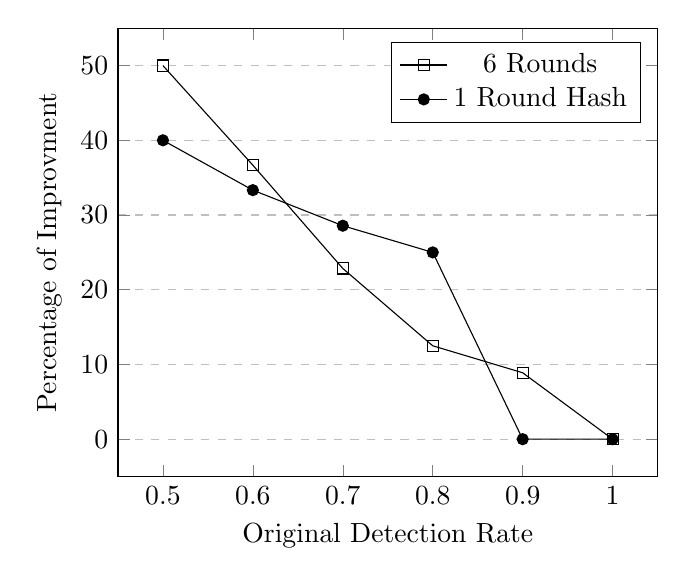
\begin{tikzpicture}
    \begin{axis}[
    xlabel={Original Detection Rate},
    ylabel={Percentage of Improvment},
    xtick={0.5,0.6,0.7,0.8,0.9,1},
    ytick={0,10,20,30,40,50,60},
    legend pos=north east,
    ymajorgrids=true,
    grid style=dashed,
    ]
    \addplot[mark=square]
    coordinates {
        (0.5,50)(0.6,36.67)(0.7,22.85)(0.8,12.5)(0.9,8.89)(1,0)
    };
    \addplot[mark=*]
    coordinates {
        (0.5,40)(0.6,33.33)(0.7,28.57)(0.8,25)(0.9,0)(1,0)
    };
    \legend{6 Rounds, 1 Round Hash}
    \end{axis}
    \end{tikzpicture}
    \caption{Gains in the Detection Rate of the MultiRound and hashing approach against the BasicSplitting $k=10,m=32$.}
    \label{fig:Improvment}
\end{figure}

Figures~\ref{fig:km2014-DR3} and \ref{fig:kmBoth-DR3} show the effect of $k$ and $m$ on the detection rate of the algorithm \ref{algo:HashNodeExactTop} for CAIDA'14 and both traces, respectively. One can see that the same trends we noted regarding the performance of algorithm \ref{algo:BasicSplitting} also hold for this case. Furthermore, these figures also show the superiority of the algorithm \ref{algo:HashNodeExactTop} over the algorithm \ref{algo:BasicSplitting} in all settings.

\begin{figure}
    \centering
    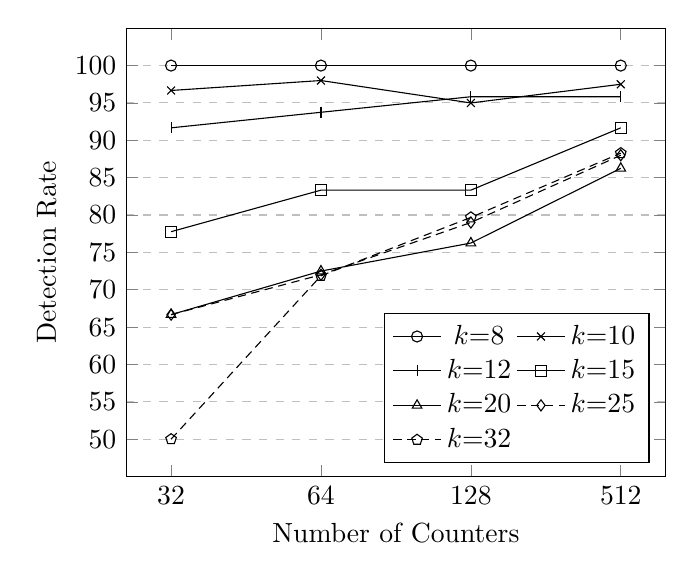
\begin{tikzpicture}
    \begin{axis}[
    xlabel={Number of Counters},
    ylabel={Detection Rate},
    xtick=data,
    xticklabels={32, 64, 128, 512},
    ytick={50,55,60,65,70,75,80,85,90,95,100},
    legend pos=south east,
    legend columns=2,
    ymajorgrids=true,
    grid style=dashed
    ]
    \addplot+[black, mark=o]
    coordinates {
        (1,100)(2,100)(3,100)(4,100)
    };
    \addlegendentry{$k$=8};
    \addplot+[black, mark=x]
    coordinates {
        (1,96.67)(2,98)(3,95)(4,97.5)
    };
    \addlegendentry{$k$=10};
    \addplot+[black, mark=|]
    coordinates {
        (1,91.67)(2,93.75)(3,95.83)(4,95.83)
    };
    \addlegendentry{$k$=12};
    \addplot+[black, mark=square]
    coordinates {
        (1,77.77)(2,83.33)(3,83.33)(4,91.67)
    };
    \addlegendentry{$k$=15};
    \addplot+[black, mark=triangle]
    coordinates {
        (1,66.67)(2,72.5)(3,76.25)(4,86.25)
    };
    \addlegendentry{$k$=20};
    \addplot+[black, mark=diamond]
    coordinates {
        (1,66.67)(2,72)(3,79)(4,88)
    };
    \addlegendentry{$k$=25};
    \addplot+[black, mark=pentagon]
    coordinates {
        (1,50)(2,71.87)(3,79.68)(4,88.28)
    };
    \addlegendentry{$k$=32};
    \end{axis}
    \end{tikzpicture}
    \caption{Effects of $k$ and $m$ on the detection rate of Algorithm \ref{algo:HashNodeExactTop} - CAIDA'14 traces.}
    \label{fig:km2014-DR3}

\end{figure}

\begin{figure}
    \centering
    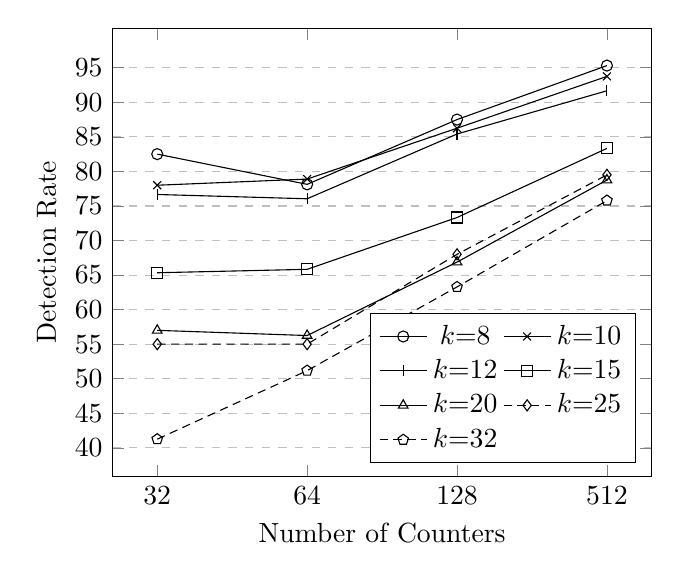
\begin{tikzpicture}
    \begin{axis}[
    xlabel={Number of Counters},
    ylabel={Detection Rate},
    xtick=data,
    xticklabels={32, 64, 128, 512},
    ytick={40,45,50,55,60,65,70,75,80,85,90,95},
    legend pos=south east,
    legend columns=2,
    ymajorgrids=true,
    grid style=dashed
    ]
    \addplot+[black, mark=o]
    coordinates {
        (1,82.5)(2,78.125)(3,87.5)(4,95.3125)
    };
    \addlegendentry{$k$=8};
    \addplot+[black, mark=x]
    coordinates {
        (1,78)(2,78.89)(3,86.25)(4,93.75)
    };
    \addlegendentry{$k$=10};
    \addplot+[black, mark=|]
    coordinates {
        (1,76.66)(2,76.04)(3,85.41)(4,91.67)
    };
    \addlegendentry{$k$=12};
    \addplot+[black, mark=square]
    coordinates {
        (1,65.334)(2,65.83)(3,73.33)(4,83.33)
    };
    \addlegendentry{$k$=15};
    \addplot+[black, mark=triangle]
    coordinates {
        (1,57)(2,56.25)(3,66.875)(4,78.75)
    };
    \addlegendentry{$k$=20};
    \addplot+[black, mark=diamond]
    coordinates {
        (1,55)(2,55)(3,68)(4,79.5)
    };
    \addlegendentry{$k$=25};
    \addplot+[black, mark=pentagon]
    coordinates {
        (1,41.25)(2,51.17)(3,63.28)(4,75.78)
    };
    \addlegendentry{$k$=32};
    \end{axis}
    \end{tikzpicture}
    \caption{Effects of $k$ and $m$ on the detection rate of Algorithm \ref{algo:HashNodeExactTop} - CAIDA'14 and CAIDA'16 traces}
    \label{fig:kmBoth-DR3}
\end{figure}

\subsection{Comparison to state of art streaming algorithms}
The RAP family of algorithms introduced recently in \cite{Ben-Basat2017} are the best performing top-$k$ streaming algorithms. As mentioned in the Introduction, these algorithms require per packet operations and complex data structures, and even when adapted to perform (i.e., dW-RAP) in line-rate they exhibit low precision rate (of about 50\%). Moreover, these algorithms are designed to address the packet rate version of the problem. 
 
Still, it is important to compare the expected performance of our algorithm that use only available counters and works well also on the traffic rate version. In \cite{Ben-Basat2017} the evaluation was done on several traces, where CAIDA’15~\cite{CAIDA15} being the dominant real-world trace. The reported experiments included a convergence period and the results depend on the number of packets in the experiment. Since our algorithms are not confined by the number of packets but by time considerations (since this is the way monitoring is done in the industry) we had to slightly modify our algorithms to allow a comparison. We changed the algorithms’ epochs and rounds to be based on the number of packets passed rather than on time units. Figure~\ref{fig:RAP} compares the detection rate of RAP and the \ref{algo:HashNodeExactTop} algorithms in this modified setting for the same CAIDA’15~\cite{CAIDA15} traces when the goal is the packet based top-$k$ flows. Note that dW-RAP uses a metadata field (flow ID) and we use very basic counters – thus in order to compare we assume that pointers to metadata have the same size as counters. One can see that for this objective and the same amount of memory there is no big difference, \ref{algo:HashNodeExactTop} performs a bit better for a small number of counters and a bit worse for large numbers. 

However, when we implemented RAP for the more relevant traffic metric the picture is a bit different.  As already mentioned in the paper, it is not straightforward to support packet size and total bit count of flows while keeping the deterministic and probabilistic bounds of RAP, so we had to modify the criterion for flow eviction to be a probabilistic function of the amount of bytes in the traffic instead of the number of packets. As depicted in Figure~\ref{fig:BWRAP}, \ref{algo:HashNodeExactTop} performs significantly better than the weighted version of RAP (denoted BW-RAP) in all settings when the number of counters is less than 512. If more than 512 counters are available then both algorithms achieve almost the same high detection rate. 

\begin{figure}
    \centering
    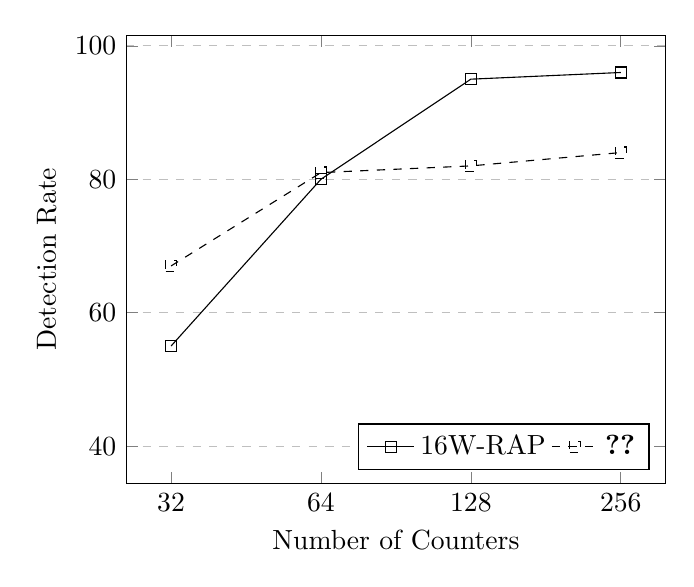
\begin{tikzpicture}
    \begin{axis}[
    xlabel={Number of Counters},
    ylabel={Detection Rate},
    xtick=data,
    xticklabels={32, 64, 128, 256},
    ytick={40,60,80,100},
    legend pos=south east,
    legend columns=2,
    ymajorgrids=true,
    grid style=dashed
    ]
    \addplot+[white, mark=none, draw=none, forget plot]
    coordinates {
        (1,40)(2,40)(3,40)(4,40)
    };
    \addplot+[black, mark=square]
    coordinates {
        (1,55)(2,80)(3,95)(4,96)
    };
    \addlegendentry{16W-RAP};
    \addplot+[black, mark=square, dashed]
    coordinates {
        (1,67)(2,81)(3,82)(4,84)
    };
    \addlegendentry{\ref{algo:HashNodeExactTop}};
    \end{axis}
    \end{tikzpicture}
    \caption{Comparison of Detection Rate for finding top-$32$ flows vs. number of counters - CAIDA'15 traces}
    \label{fig:RAP}

\end{figure}

\begin{figure}
    \centering
    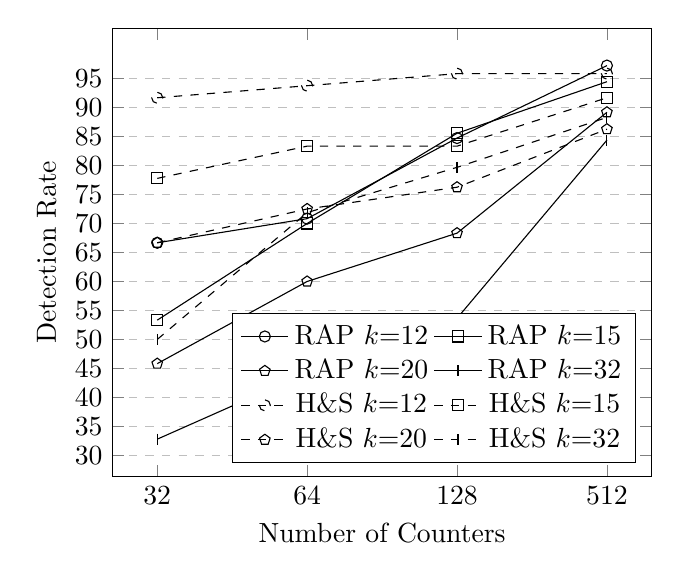
\begin{tikzpicture}
    \begin{axis}[
    xlabel={Number of Counters},
    ylabel={Detection Rate},
    xtick=data,
    xticklabels={32, 64, 128, 512},
    ytick={30,35,40,45,50,55,60,65,70,75,80,85,90,95},
    legend pos=south east,
    legend columns=2,
    ymajorgrids=true,
    grid style=dashed
    ]
    \addplot+[black, mark=o]
    coordinates {
        (1,66.67)(2,70.83)(3,84.72)(4,97.22)
    };
    \addlegendentry{RAP $k$=12};
    \addplot+[black, mark=square]
    coordinates {
        (1,53.33)(2,70)(3,85.55)(4,94.44)
    };
    \addlegendentry{RAP $k$=15};
    \addplot+[black, mark=pentagon]
    coordinates {
        (1,45.83)(2,60)(3,68.33)(4,89.17)
    };
    \addlegendentry{RAP $k$=20};
    \addplot+[black, mark=|]
    coordinates {
        (1,32.81)(2,44.27)(3,53.65)(4,84.37)
    };
    \addlegendentry{RAP $k$=32};
    \addplot+[black, mark=o, dashed]
    coordinates {
        (1,91.67)(2,93.75)(3,95.83)(4,95.83)
    };
    \addlegendentry{H\&S $k$=12};
    \addplot+[black, mark=square, dashed]
    coordinates {
        (1,77.77)(2,83.33)(3,83.33)(4,91.67)
    };
    \addlegendentry{H\&S $k$=15};
    \addplot+[black, mark=pentagon, dashed]
    coordinates {
        (1,66.67)(2,72.5)(3,76.25)(4,86.25)
    };
    \addlegendentry{H\&S $k$=20};
    \addplot+[black, mark=|, dashed]
    coordinates {
        (1,50)(2,71.87)(3,79.68)(4,88.28)
    };
    \addlegendentry{H\&S $k$=32};
    \end{axis}
    \end{tikzpicture}
    \caption{Comparison of \ref{algo:HashNodeExactTop} and BW-RAP algorithms - CAIDA'14 and CAIDA'16 traces}
    \label{fig:BWRAP}

\end{figure}
